% =================================================================
% CHAPTER 1: INTRODUCTION
% =================================================================
\chapter{Introduction} \label{chap:intro}

This chapter provides a brief introduction to the topic associated with the work carried out during the dissertation period. Firstly, a contextualization is given, followed by a presentation of the research question and the main motivations for carrying out this study. The main objectives of this dissertation will also be outlined, as well as the methodology used to achieve them. Finally, the structure of the dissertation is presented.
\section{Context} \label{sec:context}

We live in an era where smart devices are everywhere, known as the Internet of Things, IoT. While the processing and storage of information are inherently digital, benefiting from the scaling of Moore's Law, the physical world remains fundamentally analogic. Physical variables such as temperature, sound and biological potentials are continuous in both time and amplitude. Consequently, the Analog-to-Digital Converter, ADC, serves as the critical interface bridging these two domains, enabling digital systems to interact with the real world.


Energy efficiency has shifted from being a secondary performance metric to a primary design constraint, many of the sensors operate on limited battery or rely on energy harvesting, where every Joule of power dissipation has a direct effect on the system's autonomy. In this landscape, the data conversion block almost always takes place as the most spender in this field, especially in sensor interfaces where the digital transmission is duty-cycled.

However, a fundamental characteristic of many environmental and physiological signals is sparsity in between pulses. Signals such as electrocardiograms, voice activity, or environmental monitoring data are spreaded in bursts in nature: they contain short periods of high information content followed by long intervals of inactivity. 



Traditional data conversion approaches, based on uniform sampling and dictated by the Nyquist-Shannon theorem, treat these silence periods with the same computational power and energetic waste as the active periods. This creates a paradigm of inefficiency the system dissipates power to generate redundant digital samples that carry no new information. Recognizing and exploiting this sparsity is the key to unlocking ultra-low-power electronic interfaces.
\begin{figure}[htbp]
  % Since \graphicspath{{figures/}} is already defined in your preamble,
  % you just need the filename, not the full path.
  \centering
  \includegraphics[width=1\textwidth]{figures/time-sparse.png} 
  \caption{Figure adapted from Jixuan Mou (a) Time-sparse signal example. (b) Continuous-time event-driven
sampling and conversion, (c) Conventional uniform sampling
and (d) Discrete-time sampling and event-driven conversion}
  \label{fig:Sparse-time}
\end{figure}

\section{Motivation and Problem Statement} \label{sec:motivation}

The energy waste in massive-scale IoT deployments and the inefficiency of conventional synchronous architectures when processing sparse data shows the need for a fundamental shift toward architectures that activate only when meaningful data events occur.


\subsection{Inefficiency of Synchronous Sampling}

Traditional Analog-to-Digital Converters operate under a fixed-rate sampling rate, dictated by a global clock signal ($f_s$). As established by the Nyquist theorem, this rate is determined by the maximum possible bandwidth of the signal, $f_s \geq 2B$. However, in many real-world applications, the signal is often active for only a fraction of the time, meaning the true information content is much lower than the theoretical maximum bandwidth suggests.

This leads to a massive waste of energy due to the fundamental relationship governing dynamic power consumption in CMOS circuits:
\begin{equation}
  P_{dynamic} = \alpha \cdot f \cdot C_{L} \cdot V_{DD}^2
\end{equation}
Where:
\begin{itemize}
  \item $P_{dynamic}$ is the dynamic power dissipated.
  \item $\alpha$ is the activity factor (or switching factor).
  \item $f$ is the clock frequency.
  \item $C_L$ is the load capacitance being switched (e.g., in the clock tree).
\end{itemize}

\subsection{Architectural Problem: Flash ADCs}
While the Flash ADC architecture is highly attractive due to its single-cycle, high-speed conversion capability, it suffers from severe limitations regarding power and area, particularly when reaching medium-to-high resolution. The number of required comparators scales exponentially with resolution ($2^N$). This exponential scaling leads directly to an increase in input capacitance and static power dissipation.

Even in low-power, synchronous designds, the dynamic power of the comparator switching is the dominant factor in the power budget.

Therefore, combining the high speed of the Flash architecture with the high power efficiency required for IoT demands a radical shift away from the synchronous clocking scheme.

\subsection{Device Limitation: The Mismatch Problem}

To mitigate the power and area issues mentioned above, designers are compelled to minimize the physical dimensions of the core devices, particularly the transistors within the comparators. However, this introduces a fundamental physical constraint:
\begin{figure}[htbp]
  % Since \graphicspath{{figures/}} is already defined in your preamble,
  % you just need the filename, not the full path.
  \centering
  \includegraphics[width=0.6\textwidth]{offset_error.png} 
  \caption{Figure adapted from [Mohammed Abdulmahdi Mohammedali / New and Accurate Self-Test Methods for Offset Error of 10-Bit SAR-ADC] show how mismatch cause offset error in ADCs.}
  \label{fig:Offset-error}
\end{figure}





The reduction of transistor size, while increasing speed and reducing capacitance, drastically increases random variations in parameters like the threshold voltage ($V_{th}$), leading to a significant Input Offset Voltage ($V_{os}$) in the comparators.

\section{Objectives and Contribution} \label{sec:objectives}

Based on the limitations identified in traditional synchronous data conversion when dealing with sparse sensor signals, the primary objective of this work is to design and implement an energy-efficient ADC architecture, so this ADC must exploit signal inactivity to achieve a significant reduction in power consumption.

\subsection{Specific Objectives}
To achieve the overall goal of developing an efficient ADC, the following specific objectives are defined for this dissertation:

\begin{enumerate}
  \item Asynchronous Architecture Design: To develop the circuit-level design of an asynchronous Flash ADC, minimizing dynamic power consumption by ensuring that power is only dissipated when an input signal event occurs.
  
  \item Offline Trimming Implementation: To implement an offline trimming mechanism capable of detecting and compensating for the input offset voltage of the comparators.
  \item Mixed-Signal Validation: To validate the complete system through analog and digital co-simulation. This validation must confirm the functionality and accuracy of both the asynchronous core and the trimming logic.
  
  \item Performance Benchmarking: To quantify the energy efficiency of the proposed design using well known figures of merit. The results must be compared against the current state of the art synchronous ADCs and relevant asynchronous solutions.
\end{enumerate}



% =================================================================
% CHAPTER 2: LITERATURE REVIEW
% =================================================================
\chapter{Literature Review} \label{chap:lit_review}

This chapter presents the state-of-the-art in Analog-to-Digital Converters, reviewing theoretical foundations and analyzing survey data to justify the proposed architecture.


% GUIDELINE: Definir as Regras do Jogo
% Antes de comparar, define como vais medir.

\section{Fundamentals of Analog-to-Digital Conversion} \label{sec:adc_fundamentals}

This section provides the theoretical background required to understand the operation and performance characterization of data converters. It covers the fundamental steps of the conversion process such as sampling, quantization, and coding.
\subsection{The Data Conversion Process}

\subsubsection{Ideal Data Conversion}
The analog-to-digital conversion process acts as the bridge between the continuous physical world and the discrete digital domain. Conceptually, it involves two distinct operations: discretization in time, sampling, and discretization in amplitude, quantization. Ideally, this process should be instantaneous and lossless within the signal bandwidth of interest.

\subsubsection{The Sampling Operation}
Sampling converts a continuous-time signal $x(t)$ into a discrete-time sequence $x[n]$. 

According to the Nyquist-Shannon sampling theorem, a band-limited signal with maximum frequency $B$ can be perfectly reconstructed if the sampling frequency $f_s$ satisfies:
\begin{equation}
  f_s \geq 2B
\end{equation}
Violating this condition results in aliasing, where high-frequency spectral components mixes into the baseband, becoming indistinguishable from the original signal.

\subsubsection{The Quantization Operation}
While sampling transforms continuous time in discrete values, quantization maps the continuous amplitude of each sample to one of a finite number of levels. An $N$-bit ADC divides the input range ($V_{ref}$) into $2^N$ discrete levels. The step size between adjacent levels is the Least Significant Bit (LSB):
\begin{equation}
  V_{LSB} = \frac{V_{ref}}{2^N}
\end{equation}
Unlike sampling quantization is non-reversible and introduces a deterministic error. This error is typically modeled as white noise added, the quantization noise with a uniform probability distribution. For an ideal quantizer, the Signal-to-Quantization-Noise Ratio (SQNR) is given by the formula:
\begin{equation}
  SQNR_{dB} \approx 6.02N + 1.76
\end{equation}



\subsubsection{Coding}
The final stage is encoding the quantized level into a binary format. The choice of coding scheme being the most common straight binary and gray code which depends on the system requirements for data processing and transmission, but does not affect the fundamental analog performance.



\subsection{Performance Metrics}

To evaluate and compare different data converters objectively, a standard set of metrics is used. These are categorized into dynamic and static parameters.

\subsubsection{Resolution and Sampling Rate}
Resolution defines the theoretical dynamic range, while the sampling rate determines the maximum signal bandwidth. However, these are nominal values the actual performance is limited by noise and non-linearities.

\subsubsection{Signal-to-Noise-Distortion Ratio (SNDR)}
Signal to noise ratio adding distortion ratio or SNDR is the primary dynamic metric. It is the ratio of the signal power to the total power of all noise and harmonic distortion components. From SNDR, the Effective Number of Bits, ENOB, is derived:
\begin{equation}
  ENOB = \frac{SNDR_{dB} - 1.76}{6.02}
\end{equation}
This value represents the true resolution of the converter at a specific input frequency.

\subsubsection{Differential and Integral Non-Linearity (DNL and INL)}
Static linearity is characterized by measuring the deviation of code transition levels from their ideal positions. The DNL measures the deviation of a single step width from the ideal 1 LSB. A DNL less than -1 LSB implies a missing code in the transfer function.
The INL is the cumulative sum of DNL errors, representing the deviation of the transfer curve from a straight line. Specific INL patterns like saw-tooth shapes can reveal systematic errors in the architecture, such as gain mismatch or non-linear biasing.

\begin{figure}[htbp]
  % Since \graphicspath{{figures/}} is already defined in your preamble,
  % you just need the filename, not the full path.
  \centering
  \includegraphics[width=0.8\textwidth]{figures/uporto.pdf} 
  \caption{DNL and INL}
  \label{fig:myfigure}
\end{figure}



\subsubsection{Offset and Gain Error}
These are linear errors, offset is a constant shift of the transfer characteristic as seen before in section ``1.2.3 Device Limitation: The Mismatch Problem``, while gain error is a deviation in the slope. Unlike non-linearity, these errors preserve the signal shape and can often be calibrated out simply.
\begin{figure}[htbp]
  % Since \graphicspath{{figures/}} is already defined in your preamble,
  % you just need the filename, not the full path.
  \centering
  \includegraphics[width=0.8\textwidth]{figures/offset_error.png} 
  \caption{Offset and Gain Error}
  \label{fig:myfigure}
\end{figure}



\subsubsection{Bit Error Rate (BER)}
BER quantifies the probability of the converter producing an incorrect digital code. This is often caused by metastability, a phenomenon where internal decision circuits fail to resolve a valid logic level within the allocated time when the input is extremely close to a decision threshold.





\section{Synchronous Architectures} \label{sec:sync_arch}

To address asynchronous ADCs we first need to address synchronous ADCs, they have a global clock signal that dictates sampling instances and synchronizes internal operations. While these architectures are highly mature and widely used, they face fundamental power efficiency trade-offs, particularly when operating at high frequencies or processing sparse data.

\subsection{Synchronous Flash ADC}
The Flash ADC is conceptually the simplest and fastest architecture, performing a complete conversion in a single clock cycle. It utilizes a resistive ladder to generate $2^N-1$ reference voltages, which are compared simultaneously to the input signal by a large bank of comparators. This parallel comparison produces a ``thermometer code``, that a digital logic block then converts into a standard binary output. Its primary limitation is the exponential increase in hardware complexity, area, and power consumption as resolution increases.
The thermometer term refers to the parallel output from the Flash ADC comparators, where '1's run up to the input voltage level like mercury in a thermometer, indicating signal strength before being converted to standard binary by an encoder



\begin{figure}[htbp]
  \centering
  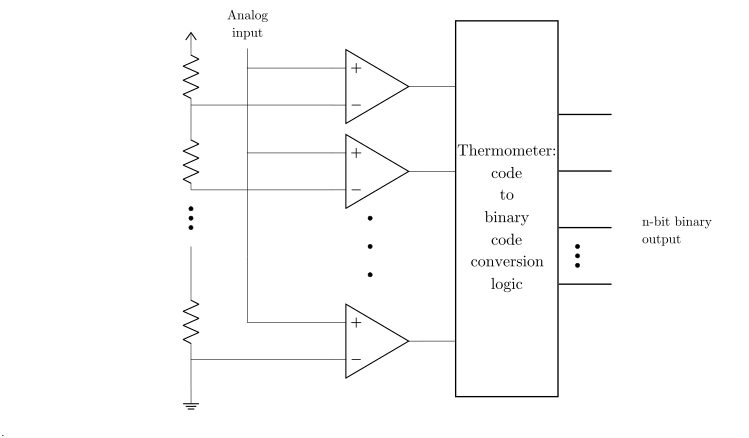
\includegraphics[width=0.8\textwidth]{figures/Flash.png} 
  \caption{Flash ADC Architecture}
  \label{fig:flash_arch}
\end{figure}

\subsection{The Power Bottleneck}
The primary drawback of the synchronous Flash architecture is its exponential scaling. Survey data clearly illustrates that high speed translates into high power in these designs, as mentioned in ``A/D converter trends: Power dissipation, scaling and digitally assisted architectures``. For example, a 6-bit 500 MS/s CMOS Flash ADC reported in 1999 already consumed 400 mW \cite{Tamba}. More extreme cases, such as a 22 GS/s 5-bit design, can consume up to 3 W \cite{Schvan_2006}.

The continuous clocking of a massive comparator bank creates a significant energy dissipation even when the input signal is static. This lack of adaptivity makes synchronous Flash architectures increasingly unsuitable for battery-powered or energy-harvesting applications.

\begin{figure}[htbp]
  \centering
  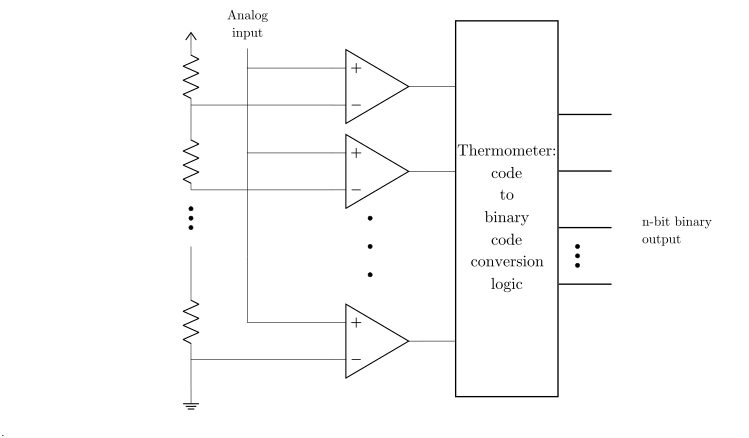
\includegraphics[width=0.8\textwidth]{figures/Flash.png} 
  \caption{Power consuption Flash ADC}
  \label{fig:flash_arch}
\end{figure}

\subsection{SAR (Successive Approximation Register)}
The SAR ADC operates using a binary search algorithm, for each sample the internal logic tests one bit at a time, starting from the most significant bit (MSB). A single comparator compares the input to the output of an internal digital to analog converter (DAC), if the input is higher, the bit is set to '1' otherwise, it is set to '0'. This process repeats for $N$ cycles. Because it uses very few active components, it is the most energy efficient choice for low speeds.



\begin{figure}[htbp]
  \centering
  \includegraphics[width=0.8\textwidth]{figures/SAR.png} 
  \caption{SAR ADC Architecture.}
  \label{fig:sar_arch}
\end{figure}

\subsection{Pipeline}
The Pipeline ADC breaks the conversion into several sequential stages, each stage resolves a few bits of information, quantizes them, and passes the remaining error,the residue, to the next stage after amplification. This approach allows the ADC to work on multiple samples concurrently, obtaining very high throughput and high resolution, the problem relies in the inherent processing latency.



\begin{figure}[htbp]
  \centering
  \includegraphics[width=0.8\textwidth]{figures/Pipeline.png} 
  \caption{Figure adapted from MPScholar: 12-bit Pipeline ADC Architecture}
  \label{fig:pipeline_arch}
\end{figure}
\paragraph{}
\paragraph{}
\paragraph{}
\paragraph{}

\subsection{Sigma-Delta ($\Sigma\Delta$)}
The $\Sigma\Delta$ architecture relies on oversampling, sampling much faster than the Nyquist rate, and noise-modulation. A modulator integrates the difference between the input signal and a feedback version of the quantized output. This process pushes the quantization noise into higher frequencies, outside the signal band of interest, a digital filter then removes the high-frequency noise, resulting in high resolution and precision.



\begin{figure}[htbp]
  \centering
  \includegraphics[width=0.8\textwidth]{Delta-sigma 1st order.png} 
  \caption{Figure adapted from MPScholar: 1st order Sigma-Delta ADC Architecture}
  \label{fig:sd_arch}
\end{figure}
\paragraph{}
\paragraph{}
\paragraph{}
\paragraph{}

\subsection{Dual-slope}
This integrating architecture measures the time required for a capacitor to charge and discharge, in the first phase, the capacitor is charged by the input voltage for a fixed period then for the second phase, it is discharged by a known reference voltage. The time it takes to return to zero is proportional to the average value of the input signal it´s highly accurate and immune to high-frequency noise but is much slower than other architectures.



\begin{figure}[htbp]
  \centering
  \includegraphics[width=0.8\textwidth]{figures/dual slope.png} 
  \caption{Figure adapted from MPScholar: Dual-slope ADC Architecture.}
  \label{fig:dual_slope_arch}
\end{figure}
\paragraph{}
\paragraph{}
\paragraph{}
\paragraph{}

\section{Asynchronous Architectures} \label{sec:async_arch}

Asynchronous, or event-driven, architectures represent a fundamental paradigm shift in data conversion, unlike synchronous ADCs, which are bound by a global cloock and the Nyquist-Shannon sampling theorem, asynchronous ADCs operate based on the signal's activity. This approach offers a more efficient alternative for processing sparse signals.

\subsection{Level-Crossing Sampling (LCS)}
The core principle behind many asynchronous ADCs is Level-Crossing Sampling (LCS). In traditional uniform sampling, the signal is captured at fixed time intervals ($T_s$), and the amplitude is quantized. In LCS, the process is inverted: the amplitude levels are fixed (quantization thresholds), and the ADC records the exact time at which the input signal crosses these thresholds.



This method is particularly powerful for signals that remain constant or change slowly over long periods. Instead of generating redundant samples that capture no new information, the LCS ADC remains idle, only producing a digital event when the signal effectively changes by more than the defined threshold.

\subsection{Asynchronous Flash ADC}
The Asynchronous Flash ADC adapts the parallel structure of a standard Flash ADC but removes the sampling clock entirely. In this architecture, the comparators are not latched by a clock, they operate in continuous time, constantly monitoring the input voltage $V_{in}$ against the reference ladder.
The event generation happens when the input signal crosses a threshold, the corresponding comparator changes it´s output state immediately, this transition triggers an asynchronous logic to generate a digital output pulse.




\subsection{Advantage}
The primary motivation for adopting asynchronous architectures is the direct relationship between signal activity and power consumption. 
In a synchronous system, the clock tree and the comparators switch at every clock cycle, regardless of whether the input is changing, the power consumption is dominated by the fixed clock frequency:
\begin{equation}
  P_{sync} \approx f_{clk} \cdot C_{total} \cdot V_{DD}^2
\end{equation}

In an asynchronous ADC, the switching frequency is replaced by the event rate. If the signal is constant or slowly varying, the comparators and digital logic remain static, leading to the following proportionality:
\begin{equation}
  P_{async} \propto \mathrm{Activity} \times V_{DD}^2
\end{equation}
This property ensures that the energy consumed is always proportional to the information content of the signal which makes these ADCs significantly more efficient for sparse signal environments, where they can achieve near-zero power during periods of inactivity.

\subsection{Comparitive Evaluation}
An analysis of state-of-the-art converters shows that asynchronous ADCs excel in energy efficiency across a wide range of sampling rates, particularly for low-to-medium bandwidths.



While Synchronous Flash ADCs are designed for peak performance at a specific frequency and suffer from a much higher power consuption caused by the continuous clocking, asynchronous designs scale their power consumption linearly with the input activity.
\begin{figure}[htbp]
  \centering
  \includegraphics[width=0.8\textwidth]{uporto-feup.pdf} 
  \caption{Difference in power between Synchronous and Asynchronous Flash ADCs.}
  \label{fig:power_comparison}
\end{figure}

\section{Figures of Merit for ADCs} \label{sec:fom_adc}

To evaluate and compare the performance of various Analog-to-Digital Converter (ADC) architectures, the scientific community relies on standardized Figures of Merit (FoM). Since ADCs vary widely in terms of resolution, speed, and power consumption, these metrics serve as a normalized benchmark to determine which design offers the best energy efficiency for a given performance target.


\subsection{Walden Figure of Merit ($FoM_W$)}
The Walden FoM is the most prevalent metric for evaluating low resolution ADCs, such as the Flash and SAR architectures. It measures the energy consumed per conversion step and is defined as:

\begin{equation}
    FoM_W = \frac{P}{2^{ENOB} \cdot f_s}
\end{equation}

Where $P$ is the power dissipation and $f_s$ is the sampling frequency. A lower Walden value indicates a more energy efficient design. This metric is particularly useful for this dissertation to demonstrate how an asynchronous architecture can reduce the numerator ($P$) by eliminating clock-related overhead.

\subsection{Schreier Figure of Merit ($FoM_S$)}
While Walden focuses on energy per step, the Schreier FoM is typically used for high-resolution ADCs where performance is limited by thermal noise ($kT/C$). It accounts for the dynamic range and bandwidth ($BW$):

\begin{equation}
    FoM_S = SNDR_{dB} + 10 \log_{10} \left( \frac{BW}{P} \right)
\end{equation}

A higher Schreier value indicates better performance. Although this work focuses on a Flash architecture, where Walden is the standard, the Schreier FoM provides a broader context regarding the physical limits of analog design.




\section{Calibration and Trimming Techniques} \label{sec:calibration}

In high-speed Flash ADCs, the accuracy of the system is fundamentally limited by the precision of the comparators. While the architecture fundamentals were established in the previous sections, practical implementations must address the non-idealities of the fabrication process, specifically the Input Offset Voltage ($V_{os}$).

\subsection{The Component Mismatch Problem}
In deep sub-micron CMOS technologies, transistors that are drawn with identical dimensions on the layout will exhibit slight differences in their electrical parameters after fabrication. This phenomenon, known as mismatch, affects the threshold voltage ($V_{th}$) and the current gain factor ($\beta$) of the differential pair in a comparator.

According to Pelgrom’s Law cited in section 2.3.3 of \cite{johns_martin_2012}, the standard deviation of the threshold voltage mismatch ($\sigma_{Vth}$) is inversely proportional to the square root of the transistor area ($W \cdot L$):

\begin{equation}
  \sigma_{V_{th}} = \frac{A_{V_{th}}}{\sqrt{W \cdot L}}
\end{equation}

Where $A_{V_{th}}$ is a technology-dependent constant. This creates a critical trade-off, to minimize offset without calibration, transistors must be made large, which increases parasitic capacitance and degrades the ADC speed and power efficiency. Therefore, small transistors are used for speed, and calibration is needed to correct the resulting offset.

\subsection{Calibration Classifications}
Calibration techniques can be broadly categorized by their timing and domain, in terms of timing there can be derived two types foreground calibration which interrupts normal operation to measure and correct errors and background calibration which operates continuously but adds significant complexity.
In terms of domain there is digital calibration that corrects the output code mathematically, whereas analog calibration adjusts the circuit biasing or load conditions to nullify the offset at the source.


For an asynchronous architecture, avoiding continuous clock activity is crucial to maintain low power during idle periods. Thus, Analog Foreground Calibration is the preferred approach.

\subsection{Resistive Trimming Techniques}
Resistive trimming aims to compensate for the imbalance in the input differential pair ($M_1, M_2$) by intentionally creating an opposing imbalance in the load resistance or the reference path.



\subsubsection{Internal Resistive Loading}
The internal resistive loading method involves placing a variable resistive network in parallel or series with the output loads of the comparator pre-amplifier stage. By digitally switching small resistors or MOS switches operating in the triode region in parallel with the load branch, the effective resistance $R_L$ is modulated. Since the gain of the pre-amplifier is defined as $A_v = g_m R_L$, changing $R_L$ on one side of the differential pair adjusts the output DC level. If the differential pair has an offset, the trimming network is adjusted to introduce an equal and opposite value to effectively zero the error. This technique is typically implemented using a binary-weighted bank of PMOS transistors as the variable resistance, where the digital control code is determined at startup and stored in a register.

\subsubsection{Resistive Reference Ladder Trimming}

The resistive reference ladder trimming technique corrects comparator offset by utilizing the main reference ladder as a calibration source \cite{yao_bulk_2011}. In this architecture, a switching network selects specific voltage taps from the resistor ladder and applies them to the bulk terminals of the input transistors M1 and M2. This approach leverages the body effect to shift the threshold voltage ($V_{th}$) of the differential pair, thereby nullifying the input-referred offset caused by process mismatch. 

As demonstrated in the simulation results of the threshold voltage ($|V_t|$) versus the ladder tap voltage ($LT$), the threshold voltage of transistors M1 and M2 increases linearly from approximately 356.5~mV to 372~mV as the calibration voltage is adjusted. In contrast, the threshold voltage of transistors M3 and M4 remains constant at approximately 356.5~mV because their bulk terminals are not connected to the tuning network. This targeted adjustment of the bulk potential for the input differential pair provides a tuning range sufficient to compensate for random process variations and ensure the accuracy of the comparator trip points.

\begin{figure}[htbp]
    \centering
    \includegraphics[width=0.7\textwidth]{VT bulk.png}
    \caption{Threshold voltage ($|V_t|$) variation of M1,2 and M3,4 as a function of the ladder tap voltage ($LT$) \cite{yao_bulk_2011}.}
    \label{fig:mismatch_correction}
\end{figure}
\paragraph{}
\paragraph{}
\paragraph{}

\paragraph{}
\paragraph{}
\subsection{Advantages of Resistive Trimming for Asynchronous ADCs}
Compared to dynamic techniques like Auto-Zeroing which requires accurate clock phases $\phi_1, \phi_2$ and storage capacitors, resistive trimming offers distinct advantages for the proposed work:
\begin{enumerate}
  \item Static Operation: Once the calibration bits are set (during the offline phase), the trimming network becomes static. It does not switch and does not require a clock, preserving the "event-driven" nature of the ADC.
  \item Speed Preservation: It does not add significant capacitive load to the high-speed nodes of the comparator, allowing for maximum bandwidth.
\end{enumerate}



\section{Related Works} \label{sec:related_works}

% =================================================================
% CHAPTER 3: FUTURE WORK PLANNING
% =================================================================
\chapter{Future Work Planning, Methodologies and Tools} \label{chap:planning}

This chapter outlines the development strategy for the dissertation, detailing the methodologies, tools, and the schedule for the remaining phases.

\section{Methodologies and Tools} \label{sec:tools}
% GUIDELINE: O "Como"
% 1. Tools: Cadence Virtuoso (Schematic/Layout), Spectre (Simulation), Verilog-A/AMS (Modeling).
% 2. Methodology: 
%  - Schematic Design based on gm/Id method.
%  - Monte Carlo Simulations (para testar o mismatch e validar o trimming).
%  - Corner Analysis (PVT - Process, Voltage, Temperature).

\section{Work Plan} \label{sec:workplan}
% GUIDELINE: O "Quando" (Baseado no teu input inicial)
% Descreve as tarefas da "Fase de Realização":
% Task 1: Schematic proposal for the asynchronous flash ADC.
% Task 2: Validation of schematic operation.
% Task 3: Characterization in PVT corners and Monte Carlo.
% Task 4: Proposal of offline trimming scheme (The Algorithm).
% Task 5: HDL implementation of the trimming strategy.
% Task 6: Full system validation and Thesis writing.
% (Se possível, insere um Gráfico de Gantt aqui).
As the work done so far was related to the first and second chapters of the dissertation, future work planning will focus on the three remaining sections. Chapter 3 will be about the mathematical formulation of the problem while Chapter 4 will involve simulation and discussion of results. Finally, in Chapter 5 are mentioned the conclusions and possible future works. To successfully complete the dissertation with respect to both time and quality, a Gantt Chart presented in Figure 3.1 was built considering the main tasks involved in the process and the expected number of days needed to conclude the tasks.


% =================================================================
% CHAPTER 4: CONCLUSIONS
% =================================================================
\chapter{Conclusions} \label{chap:conclusions}

This document presented the preparatory work for the design of an Asynchronous Flash ADC with calibration. The literature review confirmed that asynchronous architectures offer superior energy efficiency for sparse signal processing, validating the research direction. The identified challenge of comparator offset will be addressed through the proposed trimming methodology, as outlined in the work plan.